\documentclass{book}
%trying to fit more on the page
\usepackage{geometry}
\geometry{a4paper, textwidth=17cm, textheight=23cm}

\usepackage{natbib}
\usepackage{listings}
\usepackage{verbatim}
\usepackage{array}
\usepackage{amsmath, amsthm}
\usepackage{graphviz}
\usepackage{graphicx}
\usepackage{makeidx}
\usepackage{glossaries}
\usepackage{hyperref} %take this out if you don't need links.
\hypersetup{
    colorlinks,%
    citecolor=black,%
    filecolor=black,%
    linkcolor=red,%
    urlcolor=blue
}

\usepackage{url}
\usepackage{float}
\usepackage{fancybox}
\newcommand{\HRule}{\rule{\linewidth}{0.5mm}}
%use of the float package allows for \begin{table}[H] which will not allow text to be placed before the image.
%\usepackage[english]{babel} % Quotes won't work without babel
%\usepackage[utf8]{inputenc}  % This is very important!
%usepackage[T1]{fontenc} % shite font
%\usepackage{tabularx}
\usepackage{multirow}
%\usepackage{pdflscape}
%\usepackage{rotating}

%\input{glossaryentries}
%\makeglossaries
%test because text is emerging before graphics in some instances.
%\raggedbottom
%\includeonly{chap1, appen1}
\begin{document}
%\title{Undergraduate Handbook}
%\author{The University of Sheffield \\ Department of Music\\}
%\date{\today}
%\maketitle

\frontmatter

\begin{titlepage}

\begin{center}


% Upper part of the page


\includegraphics[scale=0.2]{tuoslogo_cmyk_hi} \\


%\textsc{\LARGE Department of Music.}\\[1.5cm]


% Title
\HRule \\[0.4cm]
{ \huge \bfseries MUS119}\\[0.4cm]

\HRule \\[1.5cm]

% Author and supervisor
\begin{minipage}{0.6\textwidth}
\begin{flushleft} \large
Introduction to Studio\\
\end{flushleft}
\end{minipage}

\vfill

% Bottom of the page
{\large \today}

\end{center}

\end{titlepage}

\tableofcontents

\mainmatter
\graphicspath{{images//}}
%\chapter{USSS toolkits}
%shown in figure~\ref{fig:artificialnatural}
%pages~\pageref{tab:opposites1}
%and form (section~\ref{section:form}, page~\pageref{section:form}).

\chapter{History of Electronic Music: Literature}
\label{literature}

\begin{itemize}

\item \citep{boulanger2000csound}
\item \citep{chadabe1997electric}
\item \citep{emmerson07}
\item \citep{emmersonsmalleygrove2001}
\item \citep{emmerson1986language}
\item \citep{emmerson2000music}
\item \citep{manning2013electronic}
\item \citep{roads1996computer}
\item \citep{russolo1986art}
\item \citep{born1995rationalizing}
\item \citep{holmes2008electronic}


\end{itemize}

%\chapter{USSS toolkits}
%shown in figure~\ref{fig:artificialnatural}
%pages~\pageref{tab:opposites1}
%and form (section~\ref{section:form}, page~\pageref{section:form}).

\chapter{Lesson plan}
\label{lessonplan}


\section{Scoring simple tunes}

\subsection{The triangle of film}
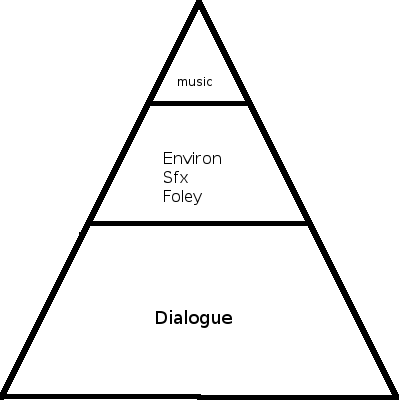
\includegraphics[scale=2.0]{triangleoffilm} 

\subsection{Simple examples}
\begin{itemize}
\item Melodic writing eg. Married life video from `Up' (a waltz in the original)
\item Score a simple melody for 16 bars. Analyse and feedback
\item Star Wars (Throne room scene: A march)
\item Examples: John Carter (2012, Stanton, music - Giacchino)
\end{itemize}

\subsection{Bring me sunshine} 
\begin{itemize}
\item Sunshine (Danny Boyle - 2007) clip 
\item Spot a piece of music from Naxos 
\item eg. Brahms1 (perhaps useful to quickly score in Sibelius and MuseScore) 
\item Add video (talk about music with video in Cubase, Premiere)
\item Introducing spotting music to clips and familiarity with Sibelius and/or MuseScore
\end{itemize}


\subsection{More spotting}
\begin{itemize}
\item Gladiator (Title 1, chapter 2 - battle scene) eg. spot with Holst Mars / compare original
\item Compose to the `battle' clip - piano only
\end{itemize}

\subsection{Harmony}
\begin{itemize}
\item Short score
\item 8 part orchestral sketch
\item Barber adagio for strings (Platoon, Stone)
\item Modes
\end{itemize}

\section{Orchestration}
\begin{itemize}
\item Woodwind (Stravinsky); Brass (Janacek, Copland): Copy in MuseScore
\item Examples. Vertigo (1958, Hitchcock - Hermann); Scott of the Antarctic (1948, Vaughan Williams); 
\item Robin Hood 1938, Korngold score; 1991, Dir: Kevin Reynolds, Music - Michael Kamen; 2010, Dir. Ridley Scott, Music - Marc Streitenfeld  
\end{itemize}

\section{Sfx}
\begin{itemize}
\item Examples: Bourne sfx; Wall-e; THX1138

\end{itemize}

\section{Writing something more experimental}
\begin{itemize}
\item This assignment could involve the use of Cubase and a more sfx / electroacoustic piece
\item The film choice could therefore be potentially `atmospheric'
\item Students may wish to be introduced to the USSStoolkit and use basic granulation to generate texture
\item Students may wish to borrow portable recorders to make their own sfx/foley
\item Foley - to picture
\item ADR - In addition to understanding the reason for ADR, in some submissions it will be important to put some of the dialogue back using students' own voices. 
\item This assignment can also be a popular music track  
\item Examples: Clockwork Orange (1971, Wendy Carlos); Bladerunner (1982, Vangelis); Social Network (2010, Trent Reznor, Atticus Ross); Forbidden Planet (1956, Barron); The Birds (1963, Hitchcock, Sala and the Trautonium)
\end{itemize}

\section{Visual Music}
\begin{itemize}
\item Examples of AV pieces where (in many cases) the composer is also the video artist. 
\item Taking this forward, students may wish to look at Processing and Blender. 
\item GEM in puredata might be useful.
\item Examples: Brett Battey; Louise Harris
\end{itemize}

\section{Opportunities: really important}
\begin{itemize}
\item South Yorkshire Filmmakers Network \url{http://syfn.org/}
\item If considering taking an special project module or extended special project with film music scoring as an outcome, scoring to materials downloaded from the internet is not allowed. You MUST find a film maker and document your process. Therefore, syfn is the place to get involved. 
\end{itemize}

\section{FAQ}
\begin{itemize}
\item Q: can I record a live ensemble? Yes, but the logistics make this almost impossible. 
\item Q: if I rip the film, I lose the dialogue and sfx,. Will I lose marks for not putting them back in. A: No, but why would you not want to make your clip as perfect as possible. We are now teaching Foley and ADR so it should be possible to approach something fully functional.
\item Q: can I rip my favourite film? A: Yes, but it will potentially be useless to score to. Hollywood isn't great for finding something really creative to work with. Better to find a finished and complete `short' so you experience scoring the whole film. 
\item Q: can I work with a film maker? A: Yes. In fact, as this is a \textbf{requirement} for MUS3040 Special Project with film. Search for South Yorkshire Filmmakers Network (syfn.org) see above.
\end{itemize}




%\chapter{USSS toolkits}
%shown in figure~\ref{fig:artificialnatural}
%pages~\pageref{tab:opposites1}
%and form (section~\ref{section:form}, page~\pageref{section:form}).

\chapter{History of film music and sound}
\label{history}

\section{Historical trends and paths}
Looking at Cooke \citeyearpar{cooke2008history} and Prendergast \citeyearpar{prendergast1992film}.

We  begin with the silence of silent films.  
Sound used to cover up the noise of the projectors and further direct the audience's concentration.

Then the temptation to add your own `imaginary' sounds when watching very realistic events. 

Sergei Eisenstein \textit{The Battleship Potemkin} (1925). 

And this very act of `perceiving' sounds by watching them happen was used by early film makers as an effect. 

Remember that even in foley, room noise is always dubbed on to give `realism'.

Sometimes `silence' is created by focusing on a single motive rather than neglecting everything. Hitchcock's \textit{The Birds} (1963) 

/textit{we need to think about what music does and therefore ask, what is film without music?}

Another reason why music appeared alongside film was because of the absence of real sound. You had actors lip syncing live from behind a screen (very acousmatic). Music ultimately `made the film feel real'. 

(page 7) Emile Reynaud's animated \textit{Pantomimes lumineuses} with music by Gaston Paulin in November 1892 as the first film music. And Georges M\'eli\`es played the piano for his own \textit{Le Voyage dans la lune}in 1902. (see Hugo for a realisation). 

Cinemas grew in the early 20th Century. 
Diegetic - often light-hearted in nature. Non-diegetic much more melodramatic. Indeed, although we don't hear it, live music was often played on set to set the mood for the actors.  

Successful production companies (still extant today) include that set up by Charles Path\'e in the early 1900s. And pianists were given cue-sheets with specific pieces of music to accompany films. Rossini \textit{William Tell} for `hurry' scenes. 

A general paradox of film music (even to this day):
\begin{quotation}
If you come out of the theatre almost unaware of the musical accompaniment to the picture you have just witnessed, the work of the musical director has been successful. Without music the present day audience would feel utterly lost. With it they should obtain an added satisfaction from the show, and still remain unconscious of the very thing which has produced that satisfaction. 

\raggedleft{\citep[16]{cooke2008history}}
\end{quotation}

Ultimately some of the key psychological features of film music boil down to simple instructions which have applied for many years. `Soft for going to happen, loud for happening'. 

\subsection{Venues and ensembles}
The rise of dedicated venues for cinema gave rise to dedicated instruments (in particular the Wurlitzer organ) and ensembles. 

\subsection{Early Epics}
Including D.W. Griffith's civil war movie \textit{The Birth of a Nation} (1915) (YT)
At three hours, it's a real epic. Original music composed by Joseph Carl Breil.

\subsection{Music for comedy}
Charlie Chaplin, Harold Lloyd, Buster Keaton.
Charlie Chaplin - \textit{Tillie's Punctured Romance} (1914) around 24:30 (YT) inside a nickelodeon (from Nickel - the 5 cent coin and odeion, a roofed theatre space).

\subsection{Music specifically for film}
Erik Satie's \textit{Entr'acte} from 1924.

Music for Sergei Eisenstein's \textit{Battleship Potemkin} (1925). With original music by Edmund Meisel but normally heard with a selection of Shostakovich. 
But Shostakovich was key to the development of film music in Russia. He worked at movie theatres in Leningrad and composed set pieces for a number of important films of the 20s. 

\subsection{The soundtrack}
Whilst there was some resistance to the addition of real-time sound, it was inevitable. 

Al Jolson in Warner Brother's \textit{The Jazz Singer} (1927) was the first ``talkie'' using the vitaphone system (a vinyl disc linked to the projector).
But \textit{The Jazz Singer} still used a compilation score (mainly Tchaikovsky - brief examples on YT) 

%Take the Jaws theme and elaborate 
%Source music and score for a scene

\section{Hollywood}

Hollywood and the studio system made film making a commercial art. MGM, Paramount, Warner Bros, Twentieth-Century Fox and RKO (Radio-Keith-Orpheum). And working conditions for composers were stressful and demanding. 

Cueing and synch was completed using a click track. Then `ducked' to enable the speech to come through. This is vital to remember if ever scoring with dialogue. 

%practical example here
% look at opera briefly

The symphonic style was unashamedly romantic - possibly a throwback from opera's success at merging music and acting, and in America, from Broadway theatre. And from Wagner, the leitmotif. 

Examples. Star Wars, Indiana Jones, Jaws. 

Citing Gorbman: Hollywood's compositional principles.
\begin{quotation}

\begin{enumerate}
\item \textit{Invisibility}: the technical apparatus of nondiegetic music must not be visible.
\item \textit{Inaudibility}: Music is not meant to be heard consciously. As such it should subordinate itself to dialogue, to visuals - i.e., to the primary vehicles of the narrative.
\item \textit{Signifier of emotion}: Soundtrack music may set specific moods and emphasize particular emotions suggested in the narrative, but first and foremost, it is a signifier of emotion itself.
\item \textit{Narrative cueing}: 
\begin{itemize}
\item \textit{referential/narrative}: music gives referential and narrative cues, e.g., indicating point of view, supplying formal demarcations, and establishing setting and characters.
\item \textit{connotative}: music `interprets' and `illustrates' narrative events.
\end{itemize}
\item \textit{Continuity}: music provides formal and rhythmic continuity - between shots, in transitions between scenes, by filling `gaps'.
\item \textit{Unity}: via repetition and variation of musical material and instrumentation, music aids in the construction of formal and narrative unity.
\item A given film score may violate an of the principles above, providing the vioilation is at the service of the other principles.

\end{enumerate}
\raggedleft{\citep[73]{gorbman1987unheard}}
\end{quotation}


\section{Key figures}
\begin{itemize}
\item Gottfried Huppertz - best known for his score to Fritz Lang's \textit{Metropolis} (1927). The story line has its Wagnerian aspects (Sci-fi meets Parsifal) and the score is very reminiscent of Wagner, Strauss and Mahler. Note the leitmotives and use of pre-existing themes such as the \textit{Dies irae} and \textit{Marseillaise}. Very descriptive writing and it's always the music which pre-figures the action and sets the scene. 
\item Max Steiner - best known for huge score of \textit{King Kong} (1933) (YT and Naxos). Also for the inside/outside use of non/diegetic music in \textit{Casablanca} (1942) with the use of Herman Hupfeld's song `As Time Goes By' (from 1931) 
\item Erich Korngold - well known for Errol Flynn blockbusters such as \textit{The Adventures of Robin Hood} (1938)
\item Franz Waxman - well known for horror music in particular \textit{The Bride of Frankenstein} (1935). Also work with Hitchcock (such as \textit{Rebecca} (1940), \textit{Suspicion} (1941) and \textit{Rear Window} (1954))
\item Alfred Newman - \textit{The Prisoner of Zenda} (1940)
\item Aaron Copland - cf. \textit{Billy the Kid} (1938) for the cowboy feel. Heard briefly in \textit{Of Mice and Men} (1940) (YT)
\item Mikl\'os R\'osa - \textit{Ben Hur} (1959)
\item Elmer Bernstein - \textit{To Kill a Mockingbird} (1962)
\item David Shire - \textit{The Taking of Pelham 123} (1974)
\item Jerry Goldsmith - \textit{The Planet of the Apes} (1968) and \textit{Escape from the Planet of the Apes} (1971)
\item Louis and Bebe Barron - \textit{The Forbidden Planet} (1956)
\item Alex North - \textit{2001: A Space Odyssey} (1968) YT but here it is interesting to note how Stanley Kubrick became so enamoured with his temp tracks that North's score was purged. 
\item Bernard Herman - beginning with \textit{Citizen Kane} (1941) and following, a close working relationship with Hitchcock. \textit{Vertigo}(1958), \textit{North by Northwest}(1959) and \textit{Psycho}(1960). N.B. whistling tune from \textit{Twisted Nerve} (1968) used in....Herman in Cook \citep[66]{cook1998analysing},
\begin{quotation}
I feel that music on the screen can seek out and intensify the inner thoughts of the characters. It can invest a scene with terror, grandeur, gaiety, or misery. It can propel narrative swiftly forward, or slow it down. It often lifts mere dialogue into the realm of poetry. Finally, it is the communicating link between the screen and the audience, reaching out and enveloping all into one single experience.
\end{quotation}

and in the United Kingdom, none other than.

\item Ralph Vaughan Williams - \textit{Scott of the Antarctic}(1948)
\item Benjamin Britten - \textit{Night Mail} (1936) - documentary and information films, but here with film composed to music and text. (YT)
\item William Walton
\item Malcolm Arnold
\item Richard Rodney Bennett - \textit{Four Weddings and a Funeral}(1994)
\item John Barry - \textit{Dances with Wolves} (1990)
and in cartoons

\item Carl Starling - WB cartoons for Daffy Duck, Donald Duck, Bugs Bunny etc. (Duck Amuck, 1953,  Vimeo) 
\end{itemize}

The list is endless and world-wide. 

\section{Sound of Cinema (BBC)}
\subsection{episode 1}
After the silents and films such as \textit{Don Juan} (1926) with discs synchronised with the picture you get works like \textit{King Kong} (1933) fully scored by Max Steiner adopting the leitmotif. For composers like Erich Wolfgang Korngold \textit{Captain Blood, 1934} the studios gave him full control over the film process. \textit{The Adventures of Robin Hood} (1938) is another prime example of his work. Korngold worked for Warner Bros. 
The BBC programme lingered on the work of Bernard Hermann naturally with \textit{Citizen Kane} then the Hitchcock collaborations: \textit{Vertigo}(1958), \textit{Psycho}(1960), \textit{Marnie}(1964) - a failure, \textit{Torn Curtain}(1965) - the film that got Hermann fired. In 1975 Hermann worked with Martin Scorsese on \textit{Taxi Driver}.

\subsection{episode 2}
Popular music in film:
\begin{itemize}
\item Scorsese's \textit{Mean Streets} using the Rolling Stones
\item John Barry, Lalo Schifrin incorporate Jazz into their music 
\item Enio Moricone creates a very singular style
\item Tarantino `finds' his music - there is no film composer
\item 1940s: Jazz with Miles Davis, 1951: \textit{A Streetcar Named Desire} with a Jazz score by \textbf{Alex North} - there's the scene with the saxophones that denoted sexual tension which was cut for strings (denoting romance not sex)
\item 1960: \textit{Beat Girl} with score by John Barry - John Barry in his own band the John Barry seven
\item Barry hit the big time with \textit{Dr. No} - orchestrating the Monty Norman theme (which had come from one his musicals). Barry was the orchestrator and arranger for which he got £250. He got a further next 11 Bond jobs and created the idea of scoring in the title track with a singing legend (like Shirley Bassey for \textit{Goldfinger}) The main tunes from these themes are then treated symphonically throughout the film.
\item 1964: Beatles' \textit{Hard Day's Night}
\item 1964: Hollywood - Richard and Robert Sherman - academy awards for film scores. Particular success with their score for P.L. Travers (author) \textit{Mary Poppins}. Their fusion of popular music and english music hall seemed entirely appropriate though many have views on D.V.Dyke's suitability for the role. Shermans went on to do the \textit{Jungle Book}
\item 1964: \textit{Fistful of Dollars} - Sergio Leone and Enio Moricone partnership. He arranged a pop record called ``pastures of plenty''. 
\item Lalo Shifrin - played with Dizzie Gillespie. Was known for his music for the TV series \textit{Mission Impossible}. He went on to score for \textit{Bullit} and \textit{Dirty Harry} (Dir: Don Siegel). 
\item 1973: Back to \textit{Mean Streets} with no composer! Lots of Phil Spector and tie-ins between the meanings on the pop record and the identities of characters.
\item 1973: George Lucas - \textit{American Graffiti} - 50s and 60s pop
\item 1977: DISCO and \textit{Saturday Night Fever} - Bee Gees and David Shire. 120bpm and tunes from the classical repertoire reorchestrated. (The example in the film is MMussorgksy's \textit{Night on a Bare Mountain})
\item More pop associated with commercial marketing of the film: 1986 ``Take my breath away'' - \textit{Top Gun}
\item 1986: David Lynch and \textit{Blue Velvet} - Angelo Badalamento. ``Mysteries of Love'' with lyrics by Lynch. Went on to collaborate on \textit{Twin Peaks}, \textit{Lost Highway} and \textit{The straight story}
\item 1992: Quentin Tarantino: \textit{Reservoir Dogs} - reliance upon the \textbf{music supervisor} - in this instance Karen Rackman. She cleared the rights for songs to be used.
\item 2003: Tarantino: reusing the Bernard Herman tune for ``Twisted Nerve'' + Moricone
\item 2006: David Arnold - \textit{Casino Royale} and \textit{Skyfall}. First song to be given an Academy Award (Adele)
 
\end{itemize}

\subsection{episode 3}
New Frontiers:
\begin{itemize}
\item \textit{Chariots of Fire} (1981, dir: Hugh Hudson). Music by Vangelis using synthesizers. Electronic score but quite close to traditional music. Produced by David Putnam.
\item 1945: Miklos Rozsa on Hitchcock's \textit{Spellbound} and the Theremin. Then again in \textit{The Lost Weekend} (dir: Billy Wilder). 
\item The Theremin - a `predictable shorthand'. 
\item \textit{Forbidden Planet} (1956, dir: Fred M. Wilcox). MGM. Sound effects came from Louis and Bebe Barron in NY. Whole score taken on. Diegetic and non-diegetic (albeit fictional). 
\item 1963 \textit{The Birds} (dir: Alfred Hitchcock) using the Trautonium by Friedrich Trautwein and Bernard Hermann.  
\item The Moog synthesizer. Walter (then Wendy) Carlos. \textit{Switched on Bach} (1968) led to Kubrick's 1971 \textit{A Clockwork Orange}. `Rape, ultra-violence and Beethoven'. 
\item Early 70s saw increased use of sound effects. Francis Ford Coppola \textit{The Conversation} (1974)
\item \textbf{Walter Murch} was a key figure here and went on to make sfx for many other films.
\item \textit{THX 1138} (1971, dir: George Lucas), again using the synthesizer.
\item \textit{Midnight Express} (1978, dir: Alan Parker) with music by Giorgio Moroder. The score achieved an Oscar.
\item Korg M1.
\item \textit{Blade Runner} (1982, dir: Ridley Scott) again had a Vangelis score. 
\item Iconic sound effects. Walter Murch again key. \textit{Apocalypse Now} (1979, dir: Francis Ford Coppola). New surround sound format for this film and increased importance of sound design.
\item Skywalker Sound, CA. Post-production. Randy Thom (worked with Walter Murch), sound designer for \textit{The Incredibles} (2004, dir: Brad Bird) received an Oscar for sound.    
\item Carter Burwell (\textit{Twilight} series) and worked exclusively with the Coen Brothers (Joel and Ethan). \textit{True Grit} (2010, dir: Coen Bros.). \textit{Barton Fink} (1991, dir: Coen Bros.) incorporating annoying sound of mosquito, recorded by sound designer Skip Lievsay.
In \textit{No Country for Old Men} (2007, dir: Coen Bros.) also score by Burwell. 
\item $\pi$ (1998, dir:  Darren Aronofsky). Music by Clint Mansell (after Pop Will Eat Itself). Thereafter \textit{Requiem for a Dream} (2000), \textit{The Fountain} (2006) and \textit{Black Swan} (2010) with the same team.  
\end{itemize}


\section{Well known films and their composers}
 
\begin{table}[H]
\begin{tabular}{|p{5.0cm}|p{8.0cm}|}
\hline
Film & Composer \\\hline
John Barry &  From Russia with Love   \\\hline
John Barry &  The Ipcress File  \\\hline
John Barry &  The Quiller Memorandum   \\\hline
John Barry &  Octopussy   \\\hline
John Barry &  Midnight Cowboy   \\\hline
John Barry &  Dances with Wolves   \\\hline
John Barry &  Out of Africa   \\\hline
John Barry &  The Specialist   \\\hline
John Barry &  Mercury Rising   \\\hline
Jerry Goldsmith &  The Man from UNCLE   \\\hline
Jerry Goldsmith &  The Waltons   \\\hline
Jerry Goldsmith &  Papillon   \\\hline
Jerry Goldsmith &  The Omen   \\\hline
Jerry Goldsmith &  Alien   \\\hline
Jerry Goldsmith &  First Blood   \\\hline
Jerry Goldsmith &  Total Recall   \\\hline
Jerry Goldsmith &  Forever Young   \\\hline
Jerry Goldsmith &  Star Trek: Nemesis   \\\hline
John Williams & Close Encounters of the Third Kind    \\\hline
John Williams & Raiders of the Lost Ark    \\\hline
John Williams & ET: The Extra Terrestrial    \\\hline
John Williams & Schindler's List    \\\hline
John Williams & Saving Private Ryan    \\\hline
John Williams & Minority Report    \\\hline
John Williams & Catch me if you can    \\\hline
John Williams & Harry Potter    \\\hline
John Williams & Star Wars    \\\hline
Danny Elfman & Spider Man    \\\hline
Hans Zimmer &  Gladiator   \\\hline
Howard Shore &  The Lord of the Rings   \\\hline
Vangelis &  Chariots of Fire   \\\hline
James Horner & Titanic    \\\hline
Alan Silvestri & Forest Gump    \\\hline

\end{tabular}
\label{tab:composersandfilms}
\end{table}

\section{Historical film music practice and analysis}

Looking at Chion \citeyearpar{chion1990} and Cook \citeyearpar{cook1998analysing}

Although sound and music should magically `meld' with the image, Chion talks about `added value'. 

Where the music is very closely linked in style, emotion and meaning it is `empathetic'. Where this is not the case the music can be `anempathetic'. 
\citep[14-15]{chion1990} gives us examples of how sound `temporalizes' image.
\begin{itemize}
\item Sustained sounds versus fluttering sounds (one is clearly more animated)
\item Predictability versus irregularity. 
\end{itemize}

Sound can augment and suggest what we're seeing (or as in horror movies) what we're not seeing. 

\section{Three modes of listening}
\begin{itemize}
\item Causal listening: `what is it?'
\item Semantic listening: `assuming a language, what is it saying?'
\item Reduced listening: `what is in the sound itself?'
\end{itemize}

Question: What do you have to work with?
\begin{itemize}
\item The sound recorded with the film
\item Foley
\item Dialogue / Dialogue replacement
\item Sfx
\item Music (diegetic or non-diegetic)
\end{itemize}

\section{Sound and silence}
Be wary of using silence (or black) as it is often perceived as though something has gone wrong. Better still to head towards the minute but keep something there.

\subsection{The Punch}
What we hear is what we haven't had time to see! \citep[61]{chion1990}

\subsection{Synchresis}
Chion's combination of \textit{syncrhonism} and \textit{synthesis}, the join between sound and image. Gestalt theories come into play here. 

\subsection{Space}
See \textit{Sonic Art: Recipes and Reasonings} for a discussion of space.  

\subsection{Time}
Sound that precedes action, sound that sums up action. Sound that raises questions.
Chion calls sound that precedes action \textit{active offscreen sound} and sound that envelops and stabilizes a scene \textit{passive offscreen sound}. Passive offscreen sound is the perfect extension of the scene and provides added value.
So you should ask yourself, `what is on screen and what is off screen?'

\subsection{Phonogeny}
Phonogeny is Chion's means to understand the quality of a sound \citep[101]{chion1990} in relation to the medium. (Note Chion's analogy of the not so beautiful women but `incredibly photogenic'). The same can be true for audio. However, current practice deprives us of the time to see and hear. This quote is worth repeating in full:

\begin{quotation}
This leads us to wonder what the disappearance of the notion of phonogeny is the symptom of. Perhaps it signals an important mutation, to our total everyday immersion in \textit{mediated acoustical reality} (sound is relayed by amplifiers and loudspeakers). The new sound reality has no difficulty supplanting unmediated acoustical reality in strength, presence, and impact, and bit by bit it is becoming the standard form of listening. It's a form of listening that is no longer perceived as a reproduction, as an image (with all this usually implies in terms of loss and distortion of reality), but as a more direct and immediate contact with the event. When an image has more presence than reality it tends to substitute for it, even as it denies its status of image.

\raggedleft{\citep[103]{chion1990}}
\end{quotation}

We now expect the hyper-real. 




\chapter{Syntax}
\label{syntax}

Michel Chion's terminology.
\begin{itemize}
\item Added Value: sound that 'naturalises' the image
\item Anempathetic sound. Sound (usually diegetic music)that plays against the plot of the film. Chion cites a scene where a radio continues to play even when the character that turned it on has died.
\item Diegetic sound is source-visible or implied by the action of the film. It can be on-screen or off-screen.
\item Non-diegetic sound is not source-visible and is usually the musical score or additional foley/sfx to the implied (diegetic) sounds.
\item Empathetic sound is usually music that is completely within the mood of the action.
\item Reduced listening: qualitative listening independent of source or meaning (also partly quantitative). Spectral listening.
\item Semantic listening: communicative content (normally language).
\item Synchresis. Relationship between audio and visual content.
\end{itemize}

\chapter{Case studies}
\label{casestudies}

\section{Case Study 1: Michael Giacchino}

Michael Giacchino (1967). website:\url{http://www.michaelgiacchinomusic.com/}. Note well his dedication to his education. He received a very thorough grounding in film, art and music. His major career boost came when he began writing for games including the well known \textit{Medal of Honor} series. He then teamed up with J.J.Abrams and wrote for a number of TV series. And through this collaboration he wrote for \textit{Star Trek} and \textit{Star Trek Into Darkness}.

His collaboration with Brad Bird have included \textit{The Incredibles}, \textit{Ratatouille}. His collaboration with Matt Reeves resulted in a score for \textit{Dawn of the Planet of the Apes}. His collaboration with Pete Doctor resulted in a score for \textit{UP}. His collaboration with Andrew Stanton resulted in a score for \textit{John Carter}.

\subsection{John Carter}
\begin{itemize}
\item Science fiction but with a Wild West slant.   
\item Horn theme. A lot of music backing the picture from simple drones to pulsing percussion.  
\item A three note theme. Open fifth (chord I to IVmin)
\item Use of Ostinati and heavy reliance upon strings.
\item Similarities with Star Trek especially in the love theme (around 1:15:00 and 1:17:30)
\end{itemize}

\section{Case Study 2: Bernard Hermann}
\begin{itemize}
\item \href{http://www.bernardherrmann.org/}
{The Society for the Appreciation of the Music of Bernard Hermann}
\item Much to be learned from \textit{Bernard Herrmann's Vertigo} (a film score handbook) by David Cooper \citep{cooper2001bernard}
\item \textit{Vertigo} is on Box of Broadcasts. 
\end{itemize}




\section{Case Study 3: Stanley Kubrick}
Ligeti's music is closely linked to the films of Stanley Kubrick. 
\begin{itemize}
\item 2001: A Space Odyssey
\begin{itemize}
\item Atmosphères (StarGate sequence and other places) 
\item Lux Aeterna (for the moon-bus scene en route to the TMA-1 monolith)
\item Requiem (Kyrie linked to the black monolith)
\item Aventures (closing scenes)
\item There are small recurrences in the film 2010.
\end{itemize}
\item The Shining uses small portions of Lontano for orchestra alongside music in a similar vein by Penderecki (Utrenja, De Natura Sonoris No.1 and No.2, and Polymorphia)
\end{itemize}




\chapter{Multimedia}
\label{multimedia}

Multimedia, music video, games, commercials. 
Sign, symbol and signified. 

Read \citep[147-173]{cook1998analysing} on Madonna's \textit{Material Girl}.



\chapter{Game audio}
\label{games}


Read \textit{Game sound: an introduction to the history, theory, and practice of video game music and sound design} \citeyearpar{collins2008game}

Think about the concepts of \textit{interactivity} and \textit{nonlinearity}. Two terms which might seem obvious at first but are fundamental to games yet frustrate the design of sound and music in games. 

Consider the notion of \textit{diegetic} and \textit{extradiegetic}. 
\begin{itemize}
\item \textit{diegetic} - a conscious interaction with the interface
\item \textit{extradiegetic} - a corporeal response to the gaming environment and experience. 
\end{itemize}

Consider the triggering of sounds. 


\chapter{Film scoring examples}
\label{examples}

More examples
\begin{itemize}
\item Forrest Gump: feather sequence. (YT)



\end{itemize}

\bibliographystyle{apalike} 
\bibliography{../../usss_coursebook/ajmbib}
%\printglossary

\backmatter
%\printindex

\end{document}
